%%%%%%%%%%%%%%%%%%%%%%%%%%%%%%%%%%%%%%%%%
% a0poster Portrait Poster
% LaTeX Template
% Version 1.0 (22/06/13)
%
% The a0poster class was created by:
% Gerlinde Kettl and Matthias Weiser (tex@kettl.de)
% 
% This template has been downloaded from:
% https://www.overleaf.com/articles/grav-redshifts/wzkygrmjsymc
%%%%%%%%%%%%%%%%%%%%%%%%%%%%%%%%%%%%%%%%%

%----------------------------------------------------------------------------------------
%	PACKAGES AND OTHER DOCUMENT CONFIGURATIONS
%----------------------------------------------------------------------------------------

\documentclass[a0,portrait]{a0poster}

\usepackage{multicol} % This is so we can have multiple columns of text side-by-side
\columnsep=100pt % This is the amount of white space between the columns in the poster
\columnseprule=3pt % This is the thickness of the black line between the columns in the poster
\usepackage[spanish,activeacute]{babel}
\usepackage{babelbib}
\usepackage{subfig}
\usepackage[svgnames]{xcolor} % Specify colors by their 'svgnames', for a full list of all colors available see here: http://www.latextemplates.com/svgnames-colors
\usepackage[hidelinks]{hyperref}
\usepackage{times} % Use the times font
%\usepackage{palatino} % Uncomment to use the Palatino font
\usepackage{amsmath}
\usepackage{graphicx} % Required for including images
\graphicspath{{figures/}} % Location of the graphics files
\usepackage{booktabs} % Top and bottom rules for table
\usepackage[font=small,labelfont=bf]{caption} % Required for specifying captions to tables and figures
\usepackage{amsfonts, amsmath, amsthm, amssymb} % For math fonts, symbols and environments
\usepackage{wrapfig} % Allows wrapping text around tables and figures

\begin{document}

%----------------------------------------------------------------------------------------
%	POSTER HEADER 
%----------------------------------------------------------------------------------------

% The header is divided into two boxes:
% The first is 75% wide and houses the title, subtitle, names, university/organization and contact information
% The second is 25% wide and houses a logo for your university/organization or a photo of you
% The widths of these boxes can be easily edited to accommodate your content as you see fit

\begin{minipage}[b]{0.75\linewidth}
\veryHuge \color{NavyBlue} \textbf{A framework for crowdrating quality evaluation in the statistical machine translation} \color{Black}\\ % Title
\\
%\Huge\textit{Prueba de Relatividad General a Grandes Escalas}\\[2cm] % Subtitle
\huge \textbf{Dmytro  Chasovskyi, Ilya Verenich}\\[0.5cm] % Author(s)
\Large Institute of Computer Science, University of Tartu, Estonia\\[0.4cm] % University/organization
\Large \texttt{\href{mailto:chasovsk@ut.ee}{\{chasovsk,ilyav\}@ut.ee}} \\
\end{minipage}
%
\begin{minipage}[b]{0.25\linewidth}

\includegraphics[scale=2]{figures/UTlogo}\qquad
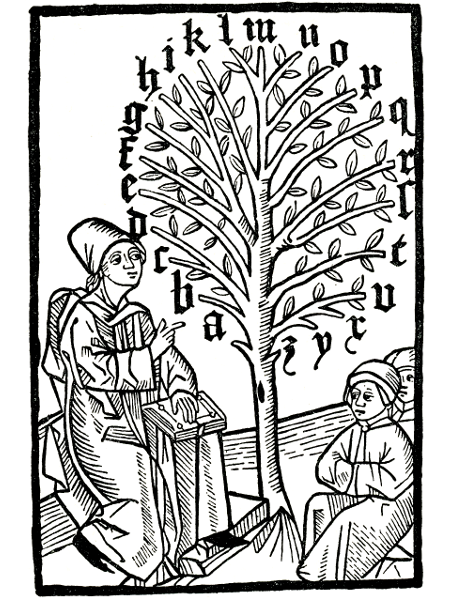
\includegraphics[scale=1.8]{figures/NLTlogo}
\end{minipage}

\vspace{1cm} % A bit of extra whitespace between the header and poster content

%----------------------------------------------------------------------------------------

\begin{multicols}{2} % This is how many columns your poster will be broken into, a portrait poster is generally split into 2 columns

%----------------------------------------------------------------------------------------
%	ABSTRACT
%----------------------------------------------------------------------------------------

%\color{DarkRed}
%
%\begin{abstract}
%
%Uno de los fen\'omenos m\'as extendidamente estudiados y considerados en la
%Cosmolog\'ia Observacional es el corrimiento al rojo. En particular, el
%corrimiento al rojo gravitacional es la 
%
%\end{abstract}

%----------------------------------------------------------------------------------------
%	INTRODUCTION
%----------------------------------------------------------------------------------------

\color{Black}
\section*{Introduction}
%There exist many tools, both open-source and closed-source, for machine translation. However, the quality of such translation is a somewhat less studied subject. In this project, we develop a framework for crowdrating quality evaluation for Estonian-English-Estonian translation.

\subsection*{Is this a good translation?}
\begin{center}\vspace{1cm}
	
\includegraphics[width=0.99\linewidth]{figures/screenshot2}
	%	\captionof{figure}{Architecture of the proposed framework.}
\end{center}


\subsection*{How to assess the translation quality?}
\begin{center}\vspace{1cm}
	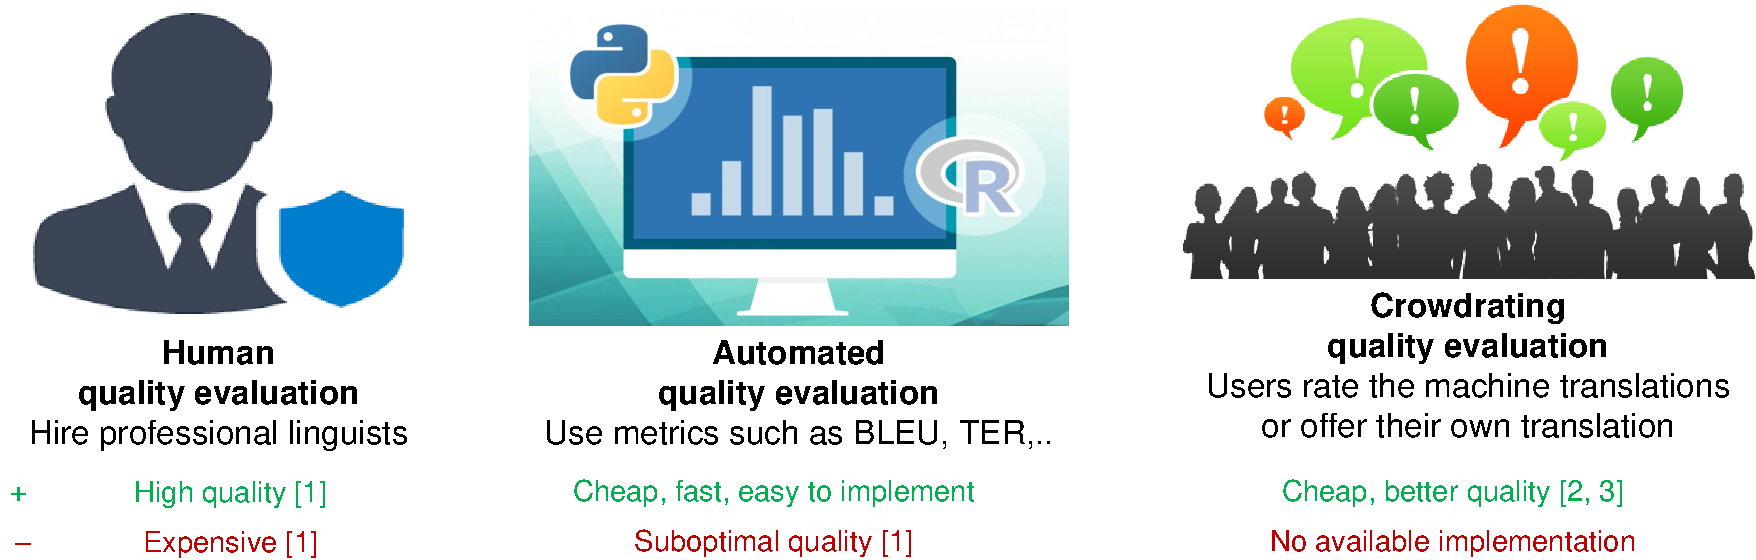
\includegraphics[width=\linewidth]{figures/qualityEvaluation}
%	\captionof{figure}{Architecture of the proposed framework.}
\end{center}

\subsection*{Contribution}
\begin{itemize}
	\item Implement a framework for crowdrating quality evaluation
	\item Improve the existing translation algorithms by using the obtained dataset of user-picked translations (work in progress)
\end{itemize}


\section*{Proposed approach}
Following are the key steps of the approach:
\begin{enumerate}
	\item User inputs a piece of text to translate
	\item The backend requests translations from translation providers
	\item User is prompted to choose the best translation among the returned results
	\item The best translation, along with the original text, are stored in the database
\end{enumerate}

\subsection*{Translation providers}
\begin{itemize}
	\item Microsoft (Bing) Translator
	\item Google Translate
	\item ``UT Translator'' from \emph{Kama} project of the Natural Language Processing Research Group -- statistical and neural network-based
\end{itemize}
%----------------------------------------------------------------------------------------
%	MATERIALS AND METHODS
%----------------------------------------------------------------------------------------


\section*{Implementation}
The source code of the implementation is available at \url{https://github.com/ChameleonTartu/masintolge}. The implementation is live at \url{masintolge.ut.ee}.

\subsection*{Architecture of the proposed framework}
\begin{center}\vspace{1cm}
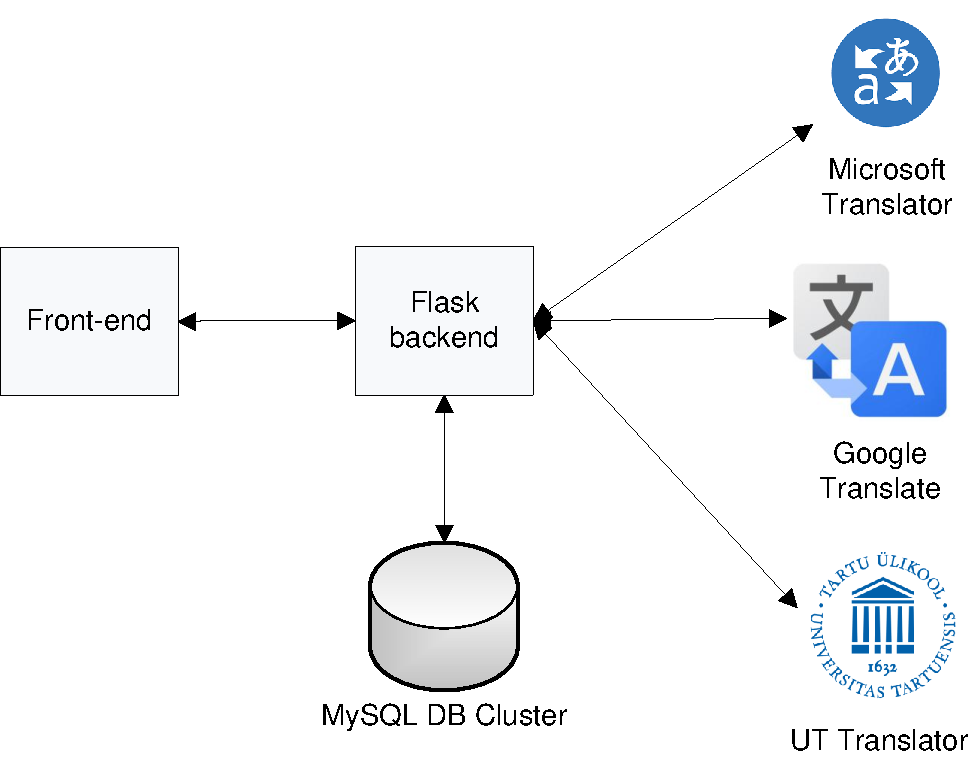
\includegraphics[width=0.8\linewidth]{figures/architecture}
%\captionof{figure}{Architecture of the proposed framework.}
\end{center}\vspace{1cm}

\subsection*{Start page with three translation variants}
\begin{center}\vspace{1cm}
	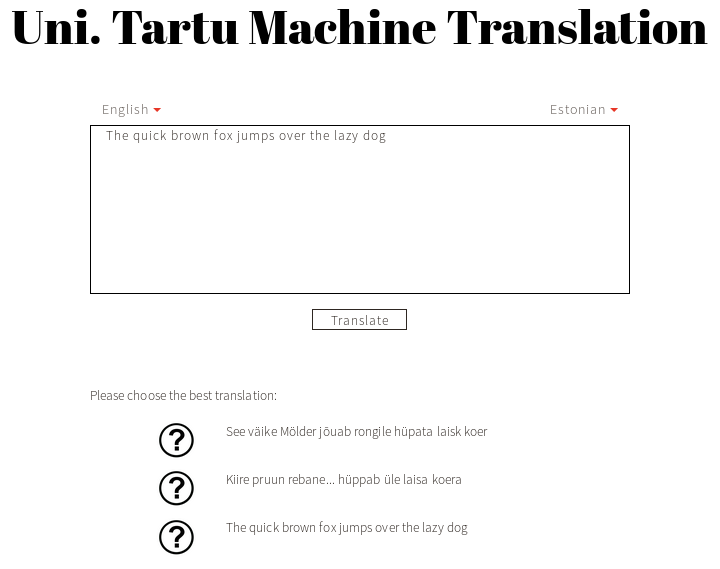
\includegraphics[width=0.9\linewidth]{figures/screenshot1}
%	\captionof{figure}{A screenshot of the implemented framework.}
\end{center}\vspace{1cm}

\subsection*{Acknowledgment of the submitted translation}
\begin{center}\vspace{1cm}
	\includegraphics[width=0.9\linewidth]{figures/screenshot3}
	%	\captionof{figure}{A screenshot of the implemented framework.}
\end{center}\vspace{1cm}

%----------------------------------------------------------------------------------------
%	CONCLUSIONS
%----------------------------------------------------------------------------------------

\section*{Future work}

\begin{itemize}
	\item Facilitating the UT translator with the crowdrated translations
\item Gamification -- users are awarded points for their contribution
\end{itemize}
 %----------------------------------------------------------------------------------------
%	REFERENCES
%----------------------------------------------------------------------------------------

\section*{Acknowledgment}
The studies of Dmytro Chasovskyi are supported by the Estonian Foreign Ministry's Development Cooperation and Humanitarian Aid funds.

\section*{References}

\begin{enumerate}
\item CBojar, O., Chatterjee, R., Federmann, C., Graham, Y., Haddow, B., Huck (2016). Findings of the 2016 conference on machine translation (WMT16). In \emph{Proceedings of the First Conference on Machine Translation (WMT)}. Vol. 2, pp. 131-198.
\item Goto, S., Lin, D., \& Ishida, T. (2014). Crowdsourcing for Evaluating Machine Translation Quality. In \emph{LREC} (pp. 3456-3463).
\item Zaidan, O. F., \& Callison-Burch, C. (2011, June). Crowdsourcing translation: Professional quality from non-professionals. In \emph{Proceedings of the 49th Annual Meeting of the Association for Computational Linguistics}. Vol. 1, pp. 1220-1229.
\end{enumerate}

%\nocite{*} % Print all references regardless of whether they were cited in the poster or not
%\bibliographystyle{plain} % Plain referencing style
%\bibliography{sample} % Use the example bibliography file %sample.bib



\end{multicols}
\end{document}